\section{Solutions}
\subsection{Choice of Input}
%das erklären was wir auch schon in der Präsentation hatten
\subsection{Learning Approaches}
%Hier sollte erwähnt werden wieso wir Evolutionär Algorithmen verwenden und keine klassischen Neuronalen Netze
%Bild mit Evolutionärer Algrotithmus allgemein, falls das noch nicht in Part 1 steht
Current methods for training spiking neural networks are often based on plasticity either spike-timing-dependent (STDP), rate-based, reward based or structural or are based on evolutionary algorithms. %hier sollte noch irgendwas dazwischen gerade halt keine idee :D
 For our purpose we chose an evolutionary approach. The basic idea behind an evolutionary or genetic algorithm is based upon biological evolution where the fitness of an individiuum decides if it survives and generates offspring. Given an initial population these algorithms are usually divided into 3 steps, as shown in Fig. \ref{evo_base}. 1) Evaluate the fitness of each individual given a fitness function f(). In our case this function is the distance achieved by running the experiment in the simulation. 2) Select the best-fit individuals for reproduction. 3) Breed and mutate indivduals to generate offsprings.

\begin{figure}[H]
	\centering
	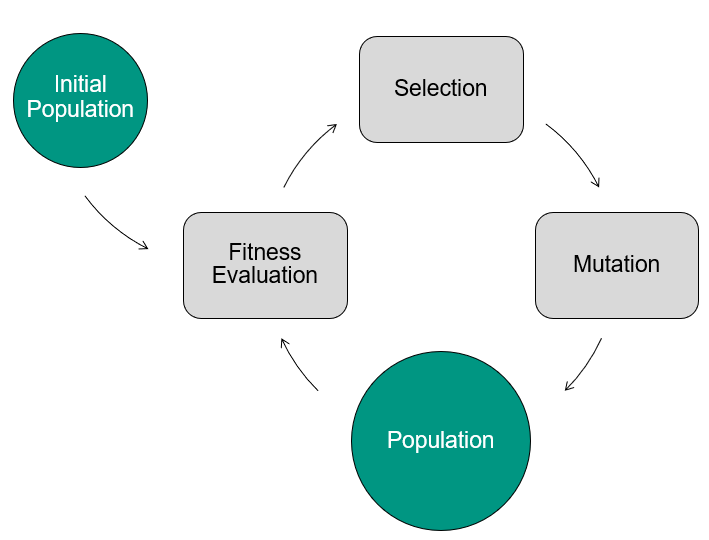
\includegraphics[width=2.2in]{img/evo_base.png}
	\DeclareGraphicsExtensions.
	\caption{General scheme of an evolutionary algorithm}
	\label{evo_base}
\end{figure}
\subsubsection{Evolutionary Strategy 1}
\subsubsection{Evolutionary Strategy 2}
The second mutation algorithm we evaluated for learning the synaptic weights of the network is based on the evolutionary strategy introduced by Salimans et al. \cite{Salimans2017EvolutionSA}. Their algorithm repeatedly executes two phases 1) Random Pertubation of the weights and evaluation the resulting parameters by running the experiment and the 2) Combining the results of the individual pertubations to compute an estimation for the stochhastic gradient decent to update the weights. The algorithm is shown below: 
\begin{algorithm}
	\caption{Evolutionary Strategy 2}
	\begin{algorithmic}[1]
		\renewcommand{\algorithmicrequire}{\textbf{Input:}}
		\REQUIRE Learning rate $\alpha$, noise standard deviation $\sigma$, initial weights $w$
		\FOR {$t = 0,1,2, ...$}
		\STATE Sample $\epsilon_{1},...,\epsilon_{n} \sim \mathcal{N}\left( 0, I \right)$
		\STATE Compute $F_{ i } = F(w_{ i } + \sigma \epsilon_{ i }= for i = 1, ..., n$
		\STATE Set $w_{ t+1 } \leftarrow  w_{ t }+ \alpha \frac{ 1 }{ n \sigma } \sum_{ j = 1 }^{ n }{F_{ j } \epsilon_{ j }  }$
		\ENDFOR
	\end{algorithmic} 
\end{algorithm}

Since the simulation in our experiment is non deterministic it should provide more stable results that the local region of a individual is evaluated more closely, before the synaptic weights are updated.
